\let\negmedspace\undefined
\let\negthickspace\undefined
\documentclass[journal]{IEEEtran}
\usepackage[a5paper, margin=10mm, onecolumn]{geometry}
\usepackage{lmodern} % Ensure lmodern is loaded for pdflatex
\usepackage{tfrupee} % Include tfrupee package

\setlength{\headheight}{1cm} % Set the height of the header box
\setlength{\headsep}{0mm}     % Set the distance between the header box and the top of the text

\usepackage{gvv-book}
\usepackage{gvv}
\usepackage{cite}
\usepackage{amsmath,amssymb,amsfonts,amsthm}
\usepackage{algorithmic}
\usepackage{graphicx}
\usepackage{textcomp}
\usepackage{xcolor}
\usepackage{txfonts}
\usepackage{listings}
\usepackage{enumitem}
\usepackage{mathtools}
\usepackage{gensymb}
\usepackage{comment}
\usepackage[breaklinks=true]{hyperref}
\usepackage{tkz-euclide} 
\usepackage{listings}
\usepackage{gvv}                                        
\def\inputGnumericTable{}                                 
\usepackage[latin1]{inputenc}                                
\usepackage{color}                                            
\usepackage{array}                                            
\usepackage{longtable}                                       
\usepackage{calc}                                             
\usepackage{multirow}                                         
\usepackage{hhline}                                           
\usepackage{ifthen}                                           
\usepackage{lscape}
\begin{document}

\bibliographystyle{IEEEtran}
\vspace{3cm}

\title{9-9.2-5}
\author{EE24BTECH11036 - Krishna Patil}
% \maketitle
% \newpage
% \bigskip
{\let\newpage\relax\maketitle}
Question: \\
 Find the area of the region bounded by the ellipse $ \frac{x^2}{4} + \frac{y^2}{9} = 1 $ . 
 \\ \\
\solution \\
using standard equation of ellipse , $ a = 2 $ , $ b = 3 $ 
\\
Area of ellipse is given by :
\begin{align}
                     \pi a b  \\
        \therefore area   &=  \pi \cdot 2 \cdot 3 \\
                          &= 6 \pi 
\end{align}
\begin{figure}[h!]
   \parindent 1px
	\centering
	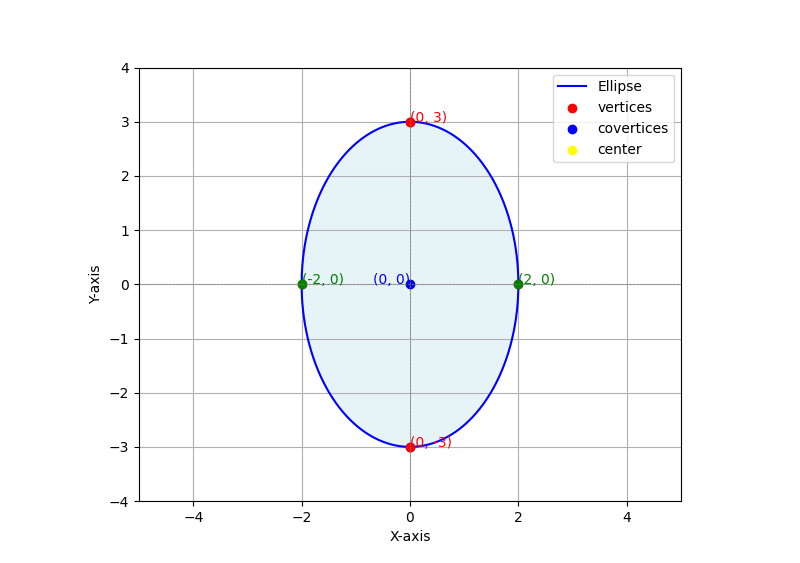
\includegraphics[width=1.0\linewidth]{figs/Figure_1.png}
   \caption{X-Y plot}
   \label{xandyplot}
\end{figure} 
\end{document}